\chapter{Phân kỳ tử ngoại và phương thuốc siêu đối xứng}

\lectureoverview{Trước khi giới thiệu toán học hình thức của siêu đối xứng, ta cần nói thật chính xác về bài toán mà nó nhằm giải quyết. Ta sẽ mô tả các phân kỳ tử ngoại cả trong không gian vị trí lẫn không gian xung lượng, suy ra hành vi khoảng cách ngắn của các propagator vô hướng và fermion bằng phân tích thứ nguyên, và ước lượng các hiệu chỉnh vòng trội lên khối lượng của một trường vô hướng. Một vòng vô hướng và một vòng fermion có cùng sự phụ thuộc bậc hai vào cutoff nhưng trái dấu nhau. Siêu đối xứng trở nên đặc biệt thuyết phục khi ta hỏi nguyên lý nào có thể khiến các hệ số ghép, bội số và khối lượng của chúng khớp nhau đủ chặt để sự triệt tiêu ấy mang tính cấu trúc chứ không phải ngẫu nhiên.}

\section{Vì sao quay lại các phân kỳ?}

Dự định ban đầu là đi ngay vào bộ máy của siêu đối xứng. Tuy nhiên, tốt hơn là hoãn phần trừu tượng lại một buổi giảng và xây dựng lại động cơ. Phần trình bày trước đó về các phân kỳ và tái chuẩn hóa khối lượng diễn ra khá nhanh, và siêu đối xứng sẽ có vẻ như một phát minh toán học tùy tiện nếu trước hết ta không thấy chính xác điều gì cần được sửa chữa.

Các giản đồ Feynman đi vào vật lý hạt theo hai cách liên hệ chặt chẽ với nhau. Quen thuộc nhất, chúng tổ chức các biên độ tán xạ. Ta chỉ rõ các hạt đi vào và đi ra rồi cộng các biên độ do mọi giản đồ ở bậc cần xét biểu diễn. Chúng cũng tổ chức việc xây dựng một \emph{Lagrangian hiệu dụng}. Ở đây, từ ``hiệu dụng'' không phải là một lời khen theo nghĩa thành công khác thường. Nó có nghĩa là mô tả chỉ gần đúng: các chi tiết khoảng cách ngắn không thể tiếp cận đã bị loại bỏ hoặc tích phân hết, và ảnh hưởng của chúng được mã hóa vào các tham số và tương tác còn lại.

Mọi mô tả như vậy đều có một miền hiệu lực. Ta có thể đặc tả miền đó bằng một khoảng cách ngắn nhất còn đáng tin, ký hiệu ở đây là \(\delta\), hoặc bằng một xung lượng lớn nhất còn đáng tin,
\begin{equation}
\Lambda\sim \delta^{-1}.
\end{equation}
Hai cutoff này không phải là hai giả thiết tách rời. Chúng là hai mô tả đối ngẫu Fourier của cùng một giới hạn tử ngoại.

\section{Một propagator, hai mô tả}

Propagator là biên độ để tạo ra hoặc chèn một hạt tại một điểm không-thời gian rồi loại bỏ hoặc phát hiện nó tại một điểm khác. Gọi hai điểm đó là \(x^\mu\) và \(y^\mu\), và viết độ tách của chúng là
\begin{equation}
\Delta^\mu=y^\mu-x^\mu.
\end{equation}
Ta dành ký hiệu chữ thường \(\delta\) cho cutoff, để không nhầm lẫn giữa độ tách và bộ điều chuẩn.

Bất biến tịnh tiến kéo theo rằng một propagator tự do chỉ phụ thuộc vào \(x\) và \(y\) thông qua \(\Delta\). Cùng đối tượng ấy có thể được biến đổi Fourier:
\begin{equation}
G(\Delta)
=\int\frac{d^4k}{(2\pi)^4}\,e^{-ik\cdot\Delta}\,\widetilde G(k).
\end{equation}

Khi câu hỏi ``Đại lượng liên hợp Fourier với vị trí là gì?'' được đặt ra cho cả lớp, câu trả lời là xung lượng. Do đó, mô tả trong không gian vị trí của một vòng như một propagator quay trở lại điểm xuất phát của nó tương đương với mô tả trong không gian xung lượng như một tích phân trên mọi xung lượng có thể lưu thông quanh vòng. Các quy tắc trong không gian xung lượng đòi hỏi phải áp đặt bảo toàn xung lượng tại mọi đỉnh; còn không gian vị trí giữ cho lập luận đếm lũy thừa hiện tại minh bạch hơn.

Sự tương đương này nhận diện bài toán tử ngoại trước cả khi ta tính toán điều gì. Trong không gian vị trí, một vòng thăm dò giới hạn đồng điểm \(\Delta\to0\). Trong không gian xung lượng, nó thăm dò giới hạn \(|k|\to\infty\). Xung lượng lớn có nghĩa là bước sóng ngắn, nên một kỳ dị khoảng cách ngắn và một phân kỳ xung lượng lớn là cùng một hiện tượng được biểu diễn trong những tọa độ khác nhau.

Bài giảng xét những lớp spin đơn giản nhất: các trường vô hướng, các trường fermion và, ở hậu cảnh, các trường gauge. Các trường vô hướng có spin không và được biểu diễn bởi trường một thành phần \(\phi(x)\). Khi bài giảng được ghi lại vào năm 2010, hạt Higgs vẫn chưa được phát hiện và được mô tả như trường vô hướng chủ yếu được trông đợi trong vật lý hạt. Bối cảnh lịch sử đó giải thích cụm từ đùa ``higgly-wiggly''; trường ấy có tính cấp thiết về mặt vật lý nhưng khi đó vẫn chưa được xác lập bằng thực nghiệm.

Đối với một trường vô hướng thực, propagator có thể được viết một cách sơ lược là
\begin{equation}
G_\phi(x,y)=\expect{0|T\!\left\{\phi(x)\phi(y)\right\}|0}
=G_\phi(\Delta).
\end{equation}
Quy ước sắp thứ tự theo thời gian và chuẩn hóa sẽ không quan trọng đối với phép đếm lũy thừa của ta. Điều quan trọng là hai phép chèn trường mô tả sự tạo ra ở một điểm và sự hủy ở điểm kia.

\begin{classroomqa}
\audiencequestion{\(x\) và \(y\) là các vị trí trong không gian hay trong không-thời gian? \lecturetimestamp{00:09:31}}
\lecturerresponse{Chúng là các điểm không-thời gian. Mỗi điểm là một bốn-vectơ. Vì vậy, propagator phụ thuộc vào độ tách bốn chiều của chúng và, trong chân không bất biến Lorentz, vào khoảng bất biến tương ứng.}
\end{classroomqa}

Một hạt spin một phần hai được mô tả bởi trường Dirac \(\psi_i(x)\). Chỉ số \(i\) là chỉ số spinor, không phải một thành phần không gian, vì vậy propagator là một ma trận:
\begin{equation}
S_{ij}(x,y)=\expect{0|T\!\left\{\psi_i(x)\bar\psi_j(y)\right\}|0}
=S_{ij}(\Delta).
\end{equation}

Một câu hỏi đặt ra cho cả lớp cho biết số thành phần: một trường Dirac bốn chiều có bốn thành phần phức. Một trường Weyl không khối lượng có thể được mô tả bằng hai thành phần phức, nên các trường tay trái và tay phải có thể được xét riêng. Đối với lập luận thứ nguyên hiện tại, điều quan trọng duy nhất là sự tồn tại của cấu trúc ma trận spinor.

Vì \(S_{ij}\) là một ma trận \(4\times4\), nó có thể được khai triển theo cơ sở các ma trận Dirac. Ban đầu ta sẽ lược bỏ các chỉ số ấy và khôi phục chúng khi chúng trở nên cần thiết. Đây không phải là khẳng định rằng cấu trúc ma trận không có mặt; đó là một sự đơn giản hóa có chủ ý trong lúc ta thiết lập luật lũy thừa tử ngoại.

\begin{classroomqa}
\audiencequestion{Khi nào trường liên hợp, hay trường có dấu dagger, phải xuất hiện trong một propagator? \lecturetimestamp{00:14:06}}
\lecturerresponse{Đối với một vô hướng thực trung hòa trong thảo luận sơ lược này, cùng một trường chứa cả toán tử tạo và toán tử hủy, nên không cần một trường dagger riêng biệt. Đối với một trường mang điện, phải phân biệt toán tử của hạt và phản hạt. Vì vậy \(\psi\), \(\psi^\dagger\), và dưới dạng hiệp biến \(\bar\psi=\psi^\dagger\gamma^0\), đóng những vai trò khác nhau đối với electron.}
\end{classroomqa}

Hạt Higgs vật lý là trung hòa, mặc dù trường Higgs cơ sở của Mô hình Chuẩn là một bộ đôi điện yếu. Bài giảng đang dùng vô hướng thực trung hòa làm mô hình cục bộ của nó; sự đơn giản hóa đó là đủ cho ước lượng tử ngoại.\editorialnote{Sự phân biệt này ngăn ví dụ vô hướng thực sơ lược bị hiểu lầm như một phát biểu đầy đủ về đa bội Higgs điện yếu.}

\section{Đơn vị tự nhiên và thứ nguyên của trường vô hướng}

Đặt \(\hbar=c=1\). Khi đó độ dài và thời gian có cùng đơn vị, còn năng lượng, khối lượng và xung lượng có đơn vị là nghịch đảo của độ dài:
\begin{equation}
[m]=[E]=[p]=L^{-1}.
\end{equation}
Tác dụng xuất hiện trong pha \(e^{iS}\), nên nó là không thứ nguyên. Một tác dụng vô hướng tiêu biểu trong bốn chiều không-thời gian là
\begin{equation}
S_\phi=\int d^4x\left[
\frac12\partial_\mu\phi\,\partial^\mu\phi
-\frac12m^2\phi^2
-\frac{\lambda}{4!}\phi^4
+\cdots\right].
\end{equation}
Các hệ số quy ước \(1/2\) và \(1/4!\) không ảnh hưởng đến phân tích thứ nguyên.

Bắt đầu với hạng động năng. Vì \([d^4x]=L^4\) và \([\partial_\mu]=L^{-1}\), điều kiện không thứ nguyên cho
\begin{align}
1
&=L^4\left(L^{-1}[\phi]\right)^2,\\
[\phi]&=L^{-1}.
\end{align}
Hạng khối lượng cho một phép kiểm tra lại:
\begin{equation}
L^4[m^2][\phi^2]
=L^4L^{-2}L^{-2}=1.
\end{equation}

Câu hỏi tiếp theo cho cả lớp là thứ nguyên của hệ số ghép bậc bốn. Nó là không thứ nguyên trong bốn chiều không-thời gian:
\begin{equation}
L^4[\lambda][\phi]^4=L^4[\lambda]L^{-4}=1
\quad\Longrightarrow\quad [\lambda]=L^0.
\end{equation}
Điều này khiến tương tác \(\phi^4\) trở nên đặc biệt trong bốn chiều. Thứ nguyên của \(\phi^6\) và các tương tác bậc cao hơn tuân theo cùng quy tắc, nhưng các hệ số ghép của chúng mang lũy thừa âm của khối lượng và vì thế báo hiệu một vai trò bị hạn chế hơn trong lý thuyết hiệu dụng.

Như vậy, chỉ riêng thứ nguyên của trường đã cho ta biết những tương tác nào có thể xuất hiện với các hệ số không thứ nguyên. Cùng phương pháp ấy sẽ xác định cả hai propagator lẫn hệ số ghép Yukawa mà không cần tính một tích phân Feynman chi tiết.

\section{Propagator vô hướng ở khoảng cách ngắn}

Trước hết hãy xét một trường vô hướng không khối lượng. Không có thang độ dài nội tại nào, nên thang duy nhất sẵn có là độ tách \(\Delta\). Bất biến tịnh tiến chỉ còn lại \(\Delta\), bất biến Lorentz rút sự phụ thuộc về độ lớn bất biến của nó, và tích của hai trường vô hướng có thứ nguyên \(L^{-2}\). Bỏ qua một hằng số số học,
\begin{equation}
G_0(\Delta)\sim\frac{1}{\Delta^2}.
\end{equation}
Không thể chỉ bằng lập luận thứ nguyên mà cố định được các hệ số như \(4\pi^2\).

Một khối lượng đưa vào độ dài Compton \(m^{-1}\). Tác động của nó được hiểu dễ nhất từ quan hệ tán sắc
\begin{equation}
E=\sqrt{\bm p^{,2}+m^2},
\qquad
E=|\bm p|\quad(m=0).
\end{equation}
Tại \(|\bm p|\gg m\), khối lượng là không đáng kể. Vì xung lượng lớn thăm dò khoảng cách ngắn, propagator có khối lượng phải tiến về hành vi \(1/\Delta^2\) của trường không khối lượng khi \(\Delta\to0\). Ở những khoảng cách lớn hơn nhiều so với \(m^{-1}\), sự truyền bị suy giảm. Bài giảng biểu diễn điều đó một cách sơ lược bởi
\begin{equation}
G_m(\Delta)\sim \frac{e^{-m|\Delta|}}{\Delta^2}.
\end{equation}
Đây cố ý không phải là một công thức chính xác. Trong không gian Euclid bốn chiều, propagator tự do chính xác tỉ lệ với \(mK_1(mr)/r\), với \(r=|\Delta|\); nó có cùng kỳ dị tử ngoại \(1/r^2\) và sự suy giảm theo hàm mũ ở khoảng cách lớn đi kèm một hệ số tiền nhân theo luật lũy thừa.\editorialnote{Dạng hàm Bessel cung cấp phần bổ sung chính xác tiêu chuẩn cho biểu thức mũ sơ lược của bài giảng và không cần thiết cho lập luận đếm lũy thừa của nó.}

Bài học then chốt rất đơn giản: khối lượng làm mềm sự truyền ở khoảng cách lớn nhưng không sửa được kỳ dị tại điểm trùng nhau. Đủ gần một điểm, mọi khối lượng hữu hạn đều trở nên không liên quan.

\section{Biểu đồ tadpole vô hướng và sự tinh chỉnh}

Tương tác bậc bốn \(\lambda\phi^4\) tạo ra một đỉnh bốn đường. Nối hai chân của nó với nhau và để lại hai chân vô hướng ngoài. Biểu đồ tadpole thu được sẽ hiệu chỉnh hệ số của \(\phi^2\), tức là khối lượng bình phương của trường vô hướng.

Khung hình được lưu lại ghi đúng thời điểm chuyển từ phân tích thứ nguyên sang hiệu chỉnh vòng này. Quan hệ tán sắc vẫn còn ở bên trái, tác dụng vô hướng và thứ nguyên của trường vẫn còn thấy một phần ở bên phải, còn biểu đồ tadpole nhỏ thì vừa xuất hiện ở giữa.

\begin{figure}[H]
\centering
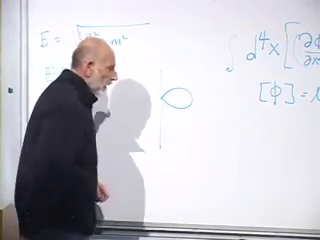
\includegraphics[width=0.72\textwidth]{lecture_03_figure_02.png}
\lectureframe{00:28:30.560}

\medskip
\begin{tikzpicture}[line width=0.8pt,scale=1.0]
  \draw[dashed] (-2.6,0) -- (0,0) -- (2.6,0);
  \fill (0,0) circle (0.055);
  \draw (0,0) .. controls (-0.85,0.7) and (-0.85,1.6) .. (0,1.6)
                .. controls (0.85,1.6) and (0.85,0.7) .. (0,0);
\end{tikzpicture}
\caption{Bảng tại thời điểm chuyển sang tự năng vô hướng, tiếp theo là bản vẽ lại sơ lược một cách dè dặt của tôpô tadpole. Ảnh chụp màn hình cho thấy chắc chắn vòng lặp, các công thức năng lượng tương đối tính và không khối lượng, cùng một phần tác dụng; các hệ số và nhãn bị che khuất không được khẳng định là nhìn thấy được.}
\end{figure}

Tại đỉnh, trường vô hướng có thể bị hấp thụ rồi phát xạ lại, trong khi hai chân còn lại truyền từ điểm đó quay về chính điểm ấy. Bỏ qua các hệ số số học và tổ hợp, hiệu chỉnh là
\begin{equation}
\delta m_\phi^2\sim \lambda G_\phi(0).
\end{equation}
Propagator tại điểm trùng là vô hạn trong gần đúng liên tục. Một lý thuyết hiệu dụng không tự nhận có hiệu lực ở khoảng cách ngắn tùy ý, nên áp đặt \(|\Delta|\geq\delta\). Khi đó
\begin{equation}
G_\phi(0)\longrightarrow G_\phi(\delta)sim\frac{1}{\delta^2},
\qquad
\delta m_\phi^2\sim\frac{\lambda}{\delta^2}sim\lambda\Lambda^2.
\end{equation}
Phân kỳ này được gọi là bậc hai vì nó chứa hai lũy thừa của cutoff xung lượng. Tích phân trong không gian xung lượng cho cùng kết luận: đóng góp quá mức đến từ xung lượng vòng lớn tùy ý. Dù thang ngắn nhất rốt cuộc được ấn định bởi đại thống nhất, hấp dẫn lượng tử hay một điều gì đó chưa từng được hình dung, chẩn đoán của lý thuyết hiệu dụng vẫn không thay đổi.

Đây là một bài toán tinh chỉnh. Nếu \(\delta\) cực kỳ nhỏ và \(\lambda\) không nhỏ đến mức phi thường, thì hiệu chỉnh bức xạ lớn hơn rất nhiều so với khối lượng bình phương của trường vô hướng quan sát được ở năng lượng thấp. Khi đó, hệ số trần và hiệu chỉnh vòng phải triệt tiêu nhau đến một số chữ số khó tin:
\begin{equation}
m_{\mathrm{physical}}^2
=m_{\mathrm{bare}}^2+\delta m_\phi^2.
\end{equation}
Propagator có khối lượng không cứu được tình hình. Ở những khoảng cách gây ra phân kỳ, \(e^{-m|\Delta|}\simeq1\). Vòng tử ngoại đã quên khối lượng từ rất lâu trước khi chạm cutoff.

\section{Thứ nguyên của fermion và propagator của chúng}

Bây giờ ta lặp lại cùng phép phân tích thứ nguyên ấy cho một fermion Dirac. Tác dụng tự do của nó là
\begin{equation}
S_\psi=\int d^4x\,
\bar\psi\left(i\gamma^\mu\partial_\mu-m\right)\psi.
\end{equation}
Các ma trận gamma là các hệ số số và không thứ nguyên. Hạng động năng chỉ chứa một đạo hàm, nên
\begin{align}
1
&=L^4[\bar\psi]L^{-1}[\psi],\\
[\psi]=[\bar\psi]&=L^{-3/2}.
\end{align}
Các lũy thừa bán nguyên không có gì đáng ngại; fermion đưa các nửa vào rất nhiều chỗ.

\begin{classroomqa}
\audiencequestion{Suy ra \([\psi]\) từ số hạng khối lượng có phải sẽ dễ hơn không? \lecturetimestamp{00:36:02}}
\lecturerresponse{Có. Số hạng khối lượng cho \(L^4L^{-1}[\bar\psi\psi]=1\), do đó \([\bar\psi\psi]=L^{-3}\) và \([\psi]=L^{-3/2}\). Phép suy ra từ hạng động năng được dùng trước vì nó vẫn có ý nghĩa trong lý thuyết không khối lượng và cho thấy vì sao khối lượng fermion xuất hiện dưới dạng \(m\), chứ không phải \(m^2\).}
\end{classroomqa}

Hai trường fermion có thứ nguyên \(L^{-3}\), vì vậy cách viết tắt gọn theo thứ nguyên trong bài giảng cho hàm truyền không khối lượng là
\begin{equation}
S(\Delta)\sim\frac{1}{|\Delta|^3}.
\end{equation}
Khôi phục cấu trúc ma trận của nó cho tử số chính xác hơn mà tính hiệp biến Lorentz đòi hỏi:
\begin{equation}
S_{ij}(\Delta)
\propto
\frac{\left(\gamma_\mu\Delta^\mu\right)_{ij}}
{\left(\Delta^2\right)^2}.
\end{equation}
Tử số bổ sung một lũy thừa chiều dài, nên mẫu số vì thế chứa bốn lũy thừa của độ tách; thứ nguyên tổng cộng vẫn là \(L^{-3}\). Cũng như với trường vô hướng, khối lượng fermion làm suy giảm hàm truyền ở độ tách lớn nhưng không làm thay đổi quy luật tỉ lệ ở khoảng cách ngắn này.

\section{Vì sao một vòng fermion kín mang dấu âm}

Bây giờ ta có thể hỏi liệu một biểu đồ fermion có thể triệt tiêu tự năng boson gây rắc rối hay không. Biểu đồ tadpole vô hướng mang dấu dương, ngoại trừ các hệ số số học dương như các lũy thừa của \(\pi\) và các hệ số tổ hợp. Một vòng fermion kín mang dấu ngược lại.

\begin{classroomqa}
\audiencequestion{Dấu trừ của vòng fermion có liên quan đến thảo luận trước đó về một phép quay trọn vòng không? \lecturetimestamp{00:40:21}}
\lecturerresponse{Nó thuộc cùng một cấu trúc dấu fermion, nhưng ở đây phép chứng minh hữu ích đi qua tính phản đối xứng dưới hoán đổi chứ không qua định hướng hình học của một vòng. Hãy cắt hai vòng, hoán đổi các hạt đồng nhất, rồi nối chúng lại. Phép hoán đổi biến hai vòng thành một và chỉ đóng góp một dấu trừ đối với fermion.}
\end{classroomqa}

Lập luận này đáng được trình bày đầy đủ. Giả sử một biểu đồ một vòng có dấu \(\sigma\), hoặc dương hoặc âm. Hai vòng đồng nhất rời nhau có dấu
\begin{equation}
\sigma^2=+1.
\end{equation}
Hãy cắt đồng thời cả hai vòng. Khi đó ta có hai hạt đồng nhất truyền giữa các chỗ cắt. Hàm sóng hai hạt thông thường của chúng là đối xứng đối với boson và phản đối xứng đối với fermion:
\begin{align}
\Psi_B(x_1,x_2)&=+\Psi_B(x_2,x_1),\\
\Psi_F(x_1,x_2)&=-\Psi_F(x_2,x_1).
\end{align}
Tính phản đối xứng này cũng giải thích nguyên lý Pauli: nếu cả hai fermion được đặt vào cùng một trạng thái, thì phép hoán vị không làm thay đổi gì về mặt vật lý nhưng lại phải đảo dấu hàm sóng, buộc nó phải bằng không.

Sau khi hoán đổi hai hạt, hãy nối lại các đường đã cắt. Về mặt tôpô, hai vòng đã trở thành một. Biên độ hai vòng trước khi hoán đổi là dương. Phép hoán đổi giữ nguyên dấu dương đối với boson và đảo dấu đối với fermion. Do đó
\begin{equation}
\begin{aligned}
\operatorname{sign}(\text{closed boson loop})&=+1,\\
\operatorname{sign}(\text{closed fermion loop})&=-1.
\end{aligned}
\end{equation}
Kết luận này là tổng quát: mỗi vòng fermion kín độc lập cung cấp một thừa số \(-1\).

\section{Vòng Yukawa}

Hãy quay lại khối lượng của trường vô hướng. Một boson không thể biến thành một fermion đơn lẻ vì tính chẵn lẻ của số fermion sẽ thay đổi. Hiệu chỉnh fermion đơn giản nhất là hạt vô hướng tách thành một cặp fermion-phản fermion, cặp này truyền quanh một vòng rồi tái hợp. Tương tác được cho bởi một ghép Yukawa,
\begin{equation}
\mathcal L_Y=-g\phi\bar\psi\psi.
\end{equation}
Đối với Higgs, các fermion có thể là quark hoặc lepton. Có hai điểm tương tác và vì thế có hai thừa số \(g\).

Biểu đồ tadpole vô hướng chỉ có một điểm, mà vị trí tổng thể của nó có thể được cố định vì bất biến tịnh tiến chỉ đơn thuần cung cấp thể tích không-thời gian. Vòng Yukawa có hai điểm. Ta có thể cố định một điểm, hoặc tương đương là cố định vị trí trung bình của chúng, nhưng phải lấy tích phân theo độ tách tương đối \(\Delta\) giữa chúng. Mỗi hàm truyền fermion đóng góp thừa số khoảng cách ngắn \(1/|\Delta|^3\), nên
\begin{equation}
\delta m_{\phi,F}^2
\sim
-g^2\int_{|\Delta|\geq\delta}d^4\Delta\,
\frac{1}{|\Delta|^6}.
\end{equation}

Sau khi đã viết hai hàm truyền, tích phân theo độ tách và hai hằng số ghép, người giảng còn hỏi cả lớp một thừa số cuối cùng. Câu trả lời là dấu trừ. Hai hàm truyền khép lại thành một vòng fermion, nên toàn bộ tích phân khoảng cách ngắn vốn dĩ dương này được nhân với \(-1\).

Phân tích thứ nguyên đã xác định được phân kỳ. Bốn lũy thừa chiều dài đến từ \(d^4\Delta\), sáu lũy thừa xuất hiện ở mẫu số, và thang chiều dài duy nhất còn lại là ngưỡng cắt:
\begin{equation}
\int_{|\Delta|\geq\delta}
\frac{d^4\Delta}{|\Delta|^6}
\sim\frac{1}{\delta^2}.
\end{equation}
Trong tọa độ xuyên tâm Euclid bốn chiều, điều này có thể được viết tường minh:
\begin{equation}
\int_{\delta}^{R}d^4\Delta\,\frac{1}{|\Delta|^6}
=2\pi^2\int_{\delta}^{R}dr\,\frac{r^3}{r^6}
=\pi^2\left(\frac{1}{\delta^2}-\frac{1}{R^2}\right).
\end{equation}
Các vết spinor và chuẩn hóa của hàm truyền làm thay đổi hệ số, chứ không làm thay đổi lũy thừa bậc hai của ngưỡng cắt.\editorialnote{Tích phân xuyên tâm là một dạng tường minh chuẩn của ước lượng theo thứ nguyên đã được thực hiện trong bài giảng. Nó được viết theo khoảng cách Euclid, nơi tính dương và phép đếm lũy thừa tử ngoại hiện ra minh bạch.}

\begin{classroomqa}
\audiencequestion{Việc đảo chiều hoặc cách chọn các cận tích phân có thể làm đổi dấu không? \lecturetimestamp{00:51:06}}
\lecturerresponse{Không. Đây không phải là một tích phân định hướng một chiều mà trong đó các cận sinh ra dấu vật lý. Nó là một tích phân trên bốn thành phần, hay gọn hơn là trên một độ đo xuyên tâm dương. Độ lớn tử ngoại của nó là dương. Đóng góp âm chỉ đến từ vòng fermion kín.}
\end{classroomqa}

\begin{classroomqa}
\audiencequestion{Hằng số ghép Yukawa \(g\) có thứ nguyên gì? \lecturetimestamp{00:51:51}}
\lecturerresponse{Nó không thứ nguyên trong bốn chiều. Vì \([\phi]=L^{-1}\) và \([\bar\psi\psi]=L^{-3}\), nên tích \(\phi\bar\psi\psi\) có thứ nguyên \(L^{-4}\), được \(d^4x\) triệt tiêu chính xác.}
\end{classroomqa}

Vì thế, hiệu chỉnh do fermion ở bậc dẫn là
\begin{equation}
\delta m_{\phi,F}^2
\sim -C_F\frac{g^2}{\delta^2}
=-C_Fg^2\Lambda^2,
\end{equation}
trong đó \(C_F>0\) chứa các hệ số số học, spin và bội số. Vòng vô hướng có dạng tương ứng
\begin{equation}
\delta m_{\phi,B}^2
\sim+C_B\frac{\lambda}{\delta^2}
=+C_B\lambda\Lambda^2.
\end{equation}
Ta vẫn chưa giải quyết được bài toán tinh chỉnh, nhưng đã tìm thấy một điều không thể thiếu: một đóng góp có cùng bậc tử ngoại và dấu ngược lại.

\section{Sự triệt tiêu đòi hỏi điều gì}

Sẽ là một ngẫu nhiên phi thường nếu các hằng số ghép không liên hệ với nhau lại tình cờ thỏa mãn
\begin{equation}
C_B\lambda=C_Fg^2
\end{equation}
với đúng độ chính xác mà một phân cấp lớn của các thang đo đòi hỏi. Bài giảng viết gọn điều này thành \(g^2=\lambda\), bỏ qua các hệ số phụ thuộc quy ước và các hệ số bội số. Một lời giải thực sự cần một cấu trúc toán học buộc quan hệ đó phải đúng, chứ không chỉ đơn thuần cho phép nó.

Đó chính là động cơ của siêu đối xứng. Siêu đối xứng liên hệ boson với fermion và ràng buộc các hằng số ghép của chúng vào những tổ hợp làm cho nhiều số hạng phân kỳ vốn nguy hiểm được triệt tiêu. Khi đó sự triệt tiêu được lặp lại trên các biểu đồ vì nó là hệ quả của một đối xứng, chứ không phải vì các tham số đã được điều chỉnh lần lượt cho từng vòng.

Sự khớp nhau của khối lượng cũng quan trọng. Nếu khối lượng boson và fermion giống hệt nhau, các hàm truyền đầy đủ của chúng có thể được ghép cặp khít nhất. Nếu các khối lượng hơi khác nhau, các kết quả hữu hạn đầy đủ không triệt tiêu chính xác, vì các hàm truyền khác nhau ở những khoảng cách cỡ bước sóng Compton của chúng. Tuy vậy, các tiệm cận khoảng cách ngắn chung của chúng vẫn có thể triệt tiêu phần phân kỳ:
\begin{equation}
\mathcal I_B(\Delta)-\mathcal I_F(\Delta)
\quad\hbox{may be finite as}\quad \Delta\to0,
\end{equation}
trong đó \(\mathcal I_B\) và \(\mathcal I_F\) ký hiệu các hàm dưới dấu tích phân đầy đủ của vòng boson và vòng fermion sau khi đã tính cả các đỉnh, tử số và các hệ số bội số. Bản thân các hàm truyền có thứ nguyên khác nhau và không phải đang bị lấy hiệu trực tiếp. Ngay cả khi các số hạng tử ngoại triệt tiêu, vẫn có thể còn lại một phần dư hữu hạn. Đây là chỗ mở ra cho siêu đối xứng gần đúng hoặc bị phá vỡ. Sự bằng nhau chính xác cho sự triệt tiêu gọn ghẽ nhất; sự phá vỡ được kiểm soát đủ tốt vẫn có thể loại bỏ thảm họa tử ngoại mà vẫn để lại sự tách khối lượng có thể quan sát được.

Vì vậy, ta đã đi tới siêu đối xứng mà vẫn chưa viết ra đại số của nó. Chuỗi lập luận đã hoàn chỉnh:
\begin{equation}
\begin{gathered}
G_\phi(\Delta)\sim \Delta^{-2},
\qquad
\delta m_{\phi,B}^2\sim+C_B\lambda\Lambda^2,\\[0.4em]
S_\psi(\Delta)\sim \Delta^{-3},
\qquad
\delta m_{\phi,F}^2\sim-C_Fg^2\Lambda^2,\\[0.4em]
\text{symmetry-enforced matching}\\
\Longrightarrow\quad
\text{quadratic divergences cancel}.
\end{gathered}
\end{equation}
Nhiệm vụ tiếp theo là hiểu nguyên lý đối xứng trừu tượng nào áp đặt những quan hệ đó và xem các ví dụ cụ thể về cách nó tác động.
